\chapter{Implementation} \label{sec:implementation}

All development of the methods detailed in this section was done using Python. 

\section{System diagram}

Figure \ref{fig:system} can help the reader gain a better understanding of how each of the materials and methods used as described in Section \ref{sec:mm} fit together.

\begin{figure}[h!]
    \centering
    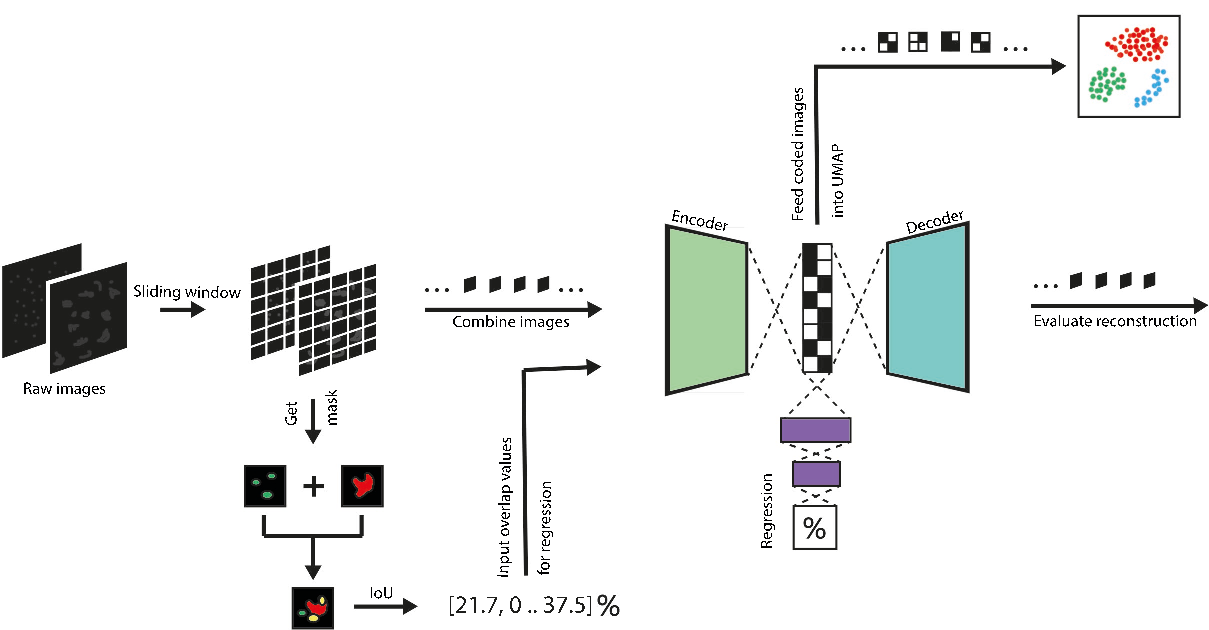
\includegraphics[width=\textwidth]{dissertation/figures/system_diagram.pdf}
    \caption{System diagram showing the project workflow and how each image is decomposed and analysed. The images are transformed into smaller patches, from which we can gain overlap labels. The images patches are then combined and used for training. On one branch, these images will be fed into an autoencoder to accomplish dimensionality reduction and evaluate the projection of this smaller data in a two-dimensional plane. On the other branch, the images will be fed in a regression model with the overlap labels in order to train a deep neural network for a regression task.}
    \label{fig:system}
\end{figure}

\section{Pre-processing}

Pre-processing steps are best explained through the diagram shown in \autoref{fig:preprocessing}. 

\begin{figure}[h!]
    \centering
    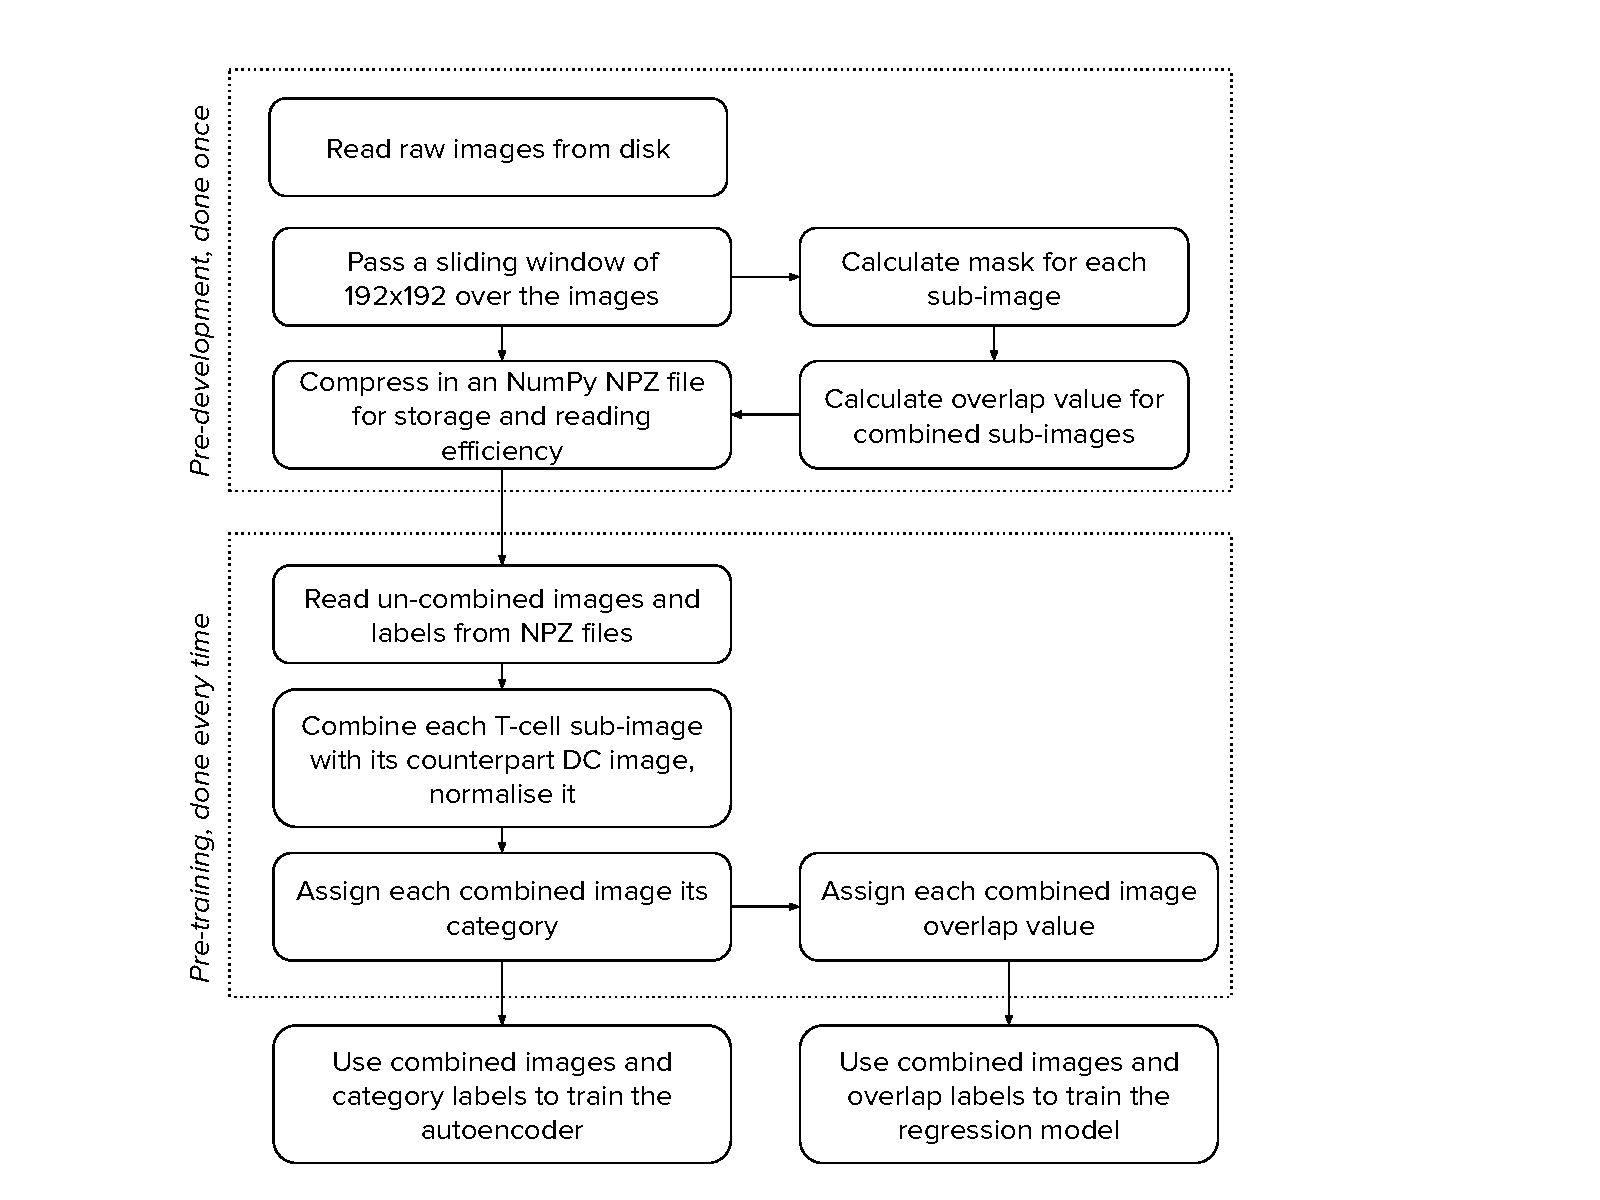
\includegraphics[width=.6\textwidth]{dissertation/figures/preprocessing_steps.pdf}
    \caption{Diagram illustrating the different steps taken for pre-processing our images. We pre-process the full images into sub-images, normalise them and combine them. We compute the overlap labels for each combined image from the mask of the T cells image and the dendritic cells image. We store the combined images and their labels in a compressed $.npz$ file. When needed, the combined images are loaded and used to train the autoencoder model. The regression model is also trained with the overlap labels. All data is shuffled before training to avoid order bias. Stimulation categories are used post-training for evaluation.}
    \label{fig:preprocessing}
\end{figure}

Images were processed with a sliding window of size $192\times192$ as we wanted a window that was large enough to contain a few cells but also wanted to make it smaller to be able to reduce individual image dimensions further. A sliding window of $192\times192$ yielded 100 patches as our images were originally of size $2048\times2048$. This meant the left and right border of the full image were cropped out. We used NumPy's compressed $.npz$ file format for writing and reading the images as they were computationally represented as multi-dimensional arrays of floating point values and it made loading the arrays much faster. It also reduced storage space by a factor of 2.5 on average. 

\section{Image segmentation}

As discussed in Section \ref{sec:dl_immunology}, performing cell segmentation from greyscale microscope images of cells has been researched and is necessary when an image contains different types of cells which have not been separately labelled in one way or another. In our case, cell segmentation did not need to be applied as the images of T cells and dendritic cells have been captured separately through fluorescent dyes. Instead, we were interested in using segmentation techniques to obtain the mask of each type of immune cell for the purposes of background correction and estimating interaction, as explained in Section \ref{sec:segmentation}.

As the immune cells in our images were bright blobs on a dark background, we hoped that obtaining masks from each image would be straightforward. This section describes the methods we explored for this task. Both k-means and thresholding methods yielded good results and their specifics are detailed below.

Furthermore, we also explored the use of a deep learning model which was developed with the purpose of segmenting biomedical data: the U-Net model. 

\subsection{\textit{k}-means colour clustering}

k-means has been shown to perform well on image segmentation by quantifying the number of colours in an image into \textit{k} clusters (\citealt{ng_kmeans}, for example). Formally, k-means aims to partition data points in an array into \textit{k} sets such that the variance between points within clusters is minimised. In our case we wanted to use k-means to transform our greyscale images of immune cells into bichrome images that we could use as masks. The following pseudocode details the process of k-means.

\begin{algorithm}[h]
    \DontPrintSemicolon
    \KwData{$I$, an array of pixel values making an image.\;
    $k$, the number of colours to partition the image's colour palette to.\;}
    \KwResult{A set of $k$ clusters.}
    \Begin{
        Initialise $k$ objects picked from $I$\;
        \While{{clusters are still changing}}
        {
           Assign each item $i$ in $I$ to the cluster with closest mean value\;
           Recompute the mean (centroid) of each cluster\;
        }
    }
    
\caption{Pseudocode for the k-means algorithm applied to image segmentation.}
\label{alg:kmeans}
\end{algorithm}

k-means clustering is conveniently offered by multiple libraries in Python. We looked at both scikit-learn's and OpenCV's k-means. scikit-learn is a general library  for machine learning tools, while OpenCV is a more specialised library built for computer vision purposes. Both their k-means functions are straightforward to initialise and use. Their performance was benchmarked in order to select the best one. The table below reports times for k-means with \textit{k}=2, 10 iterations, and each of the random and optimised methods of initialising centroids.

\begin{table}[h]
\centering
\caption{CPU times for OpenCV's and scikit-learn's k-means tool ran on 1,000 samples of $192\times192$ pixels with different methods of initialising centroids.  The computation was ran on a 2015 MacBook Pro with 2.7 GHz i5 core and 8 GB memory.}
\begin{tabular}{l|r|r}
\rowcolor[HTML]{EFEFEF} 
\textbf{Initialisation} & \textbf{OpenCV} & \textbf{scikit-learn} \\ \hline
Random                                   & 18.9s       & 165s \\ \hline
k-means++  & 29.3s   & 139s   \\ 
\end{tabular}
\end{table}

As we can see OpenCV outperforms scikit-learn in all cases. OpenCV for Python is a wrapper library around the original OpenCV code built in C++, which gives it a boost in performance. OpenCV's k-means was thus selected. Initially, k-means centers were initialised randomly in development for the performance. However, during validation it was found that this method of initialisation was yielding highly different results for the intersection-over-union metric at every run, causing issues in model predictions. Hence, some speed was traded for consistency and the k-means++ center initialisation method was selected instead. 

\subsection{Thresholding}

An alternative to k-means in the case of black-and-white image segmentation is thresholding. We decided to explore this option as it could have performance improvements compared to k-means. 

Thresholding refers to the process of converting a greyscale image to a binary image of pixels. Pixels above a set threshold are set to 1, and the pixels below that threshold are set to 0. Thresholding depends on pixel distribution analysis. Usually, thresholding works well for images which have different peaks of pixel values in their distribution. We can then pick the value which seems to separate out the two peaks as our threshold. However, in the case of our images we had one visible peak of pixel values and could not identify a viable threshold from the histogram. Figure \ref{fig:thresholdhist} illustrates this.

\begin{figure}[h]
    \centering
    \begin{subfigure}{0.45\textwidth}
        \centering
        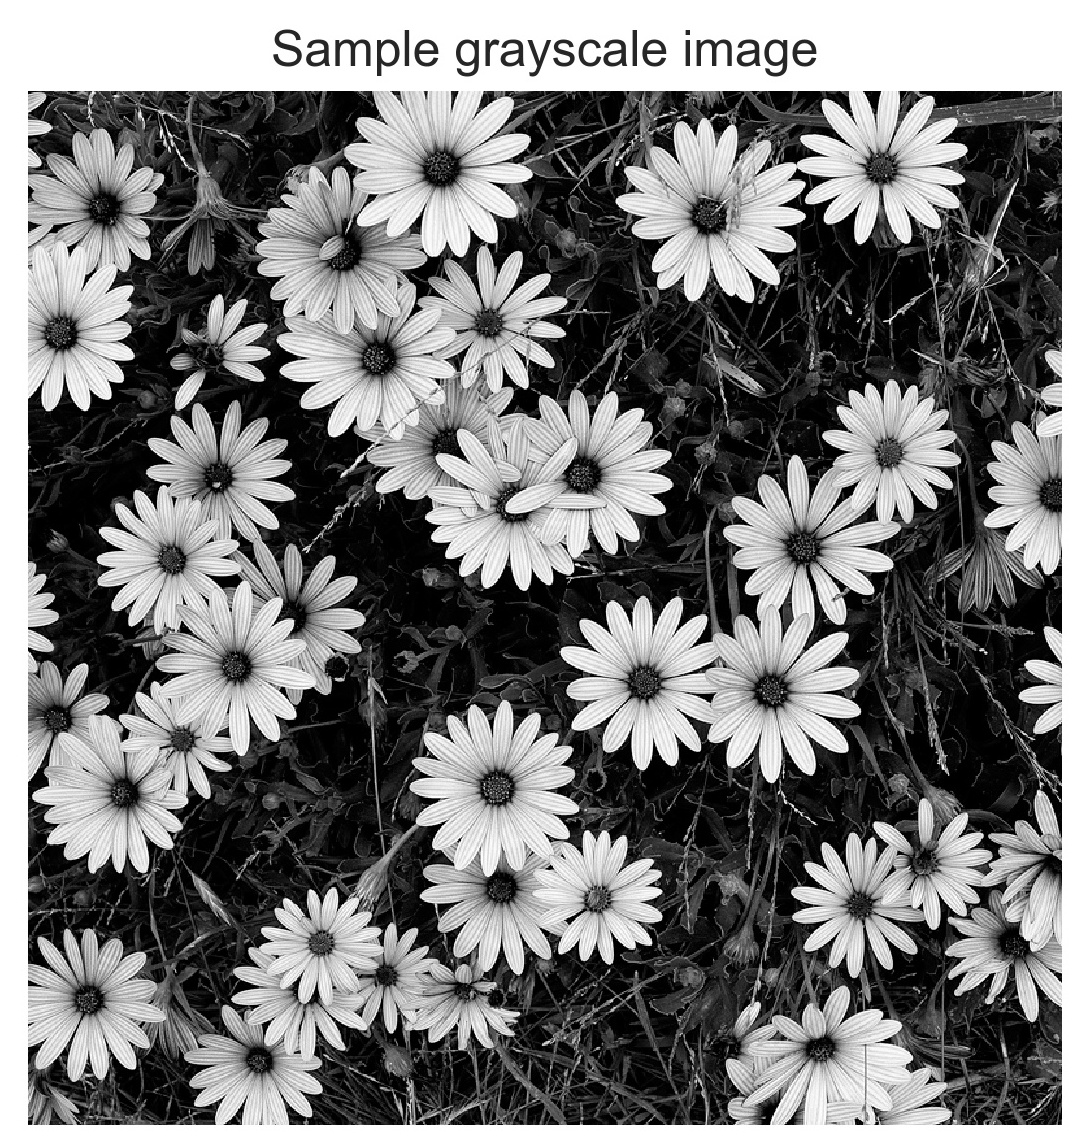
\includegraphics[width=0.6\textwidth]{dissertation/figures/sample_grayscale.jpg}
    \end{subfigure}
    \begin{subfigure}{0.45\textwidth}
        \centering
        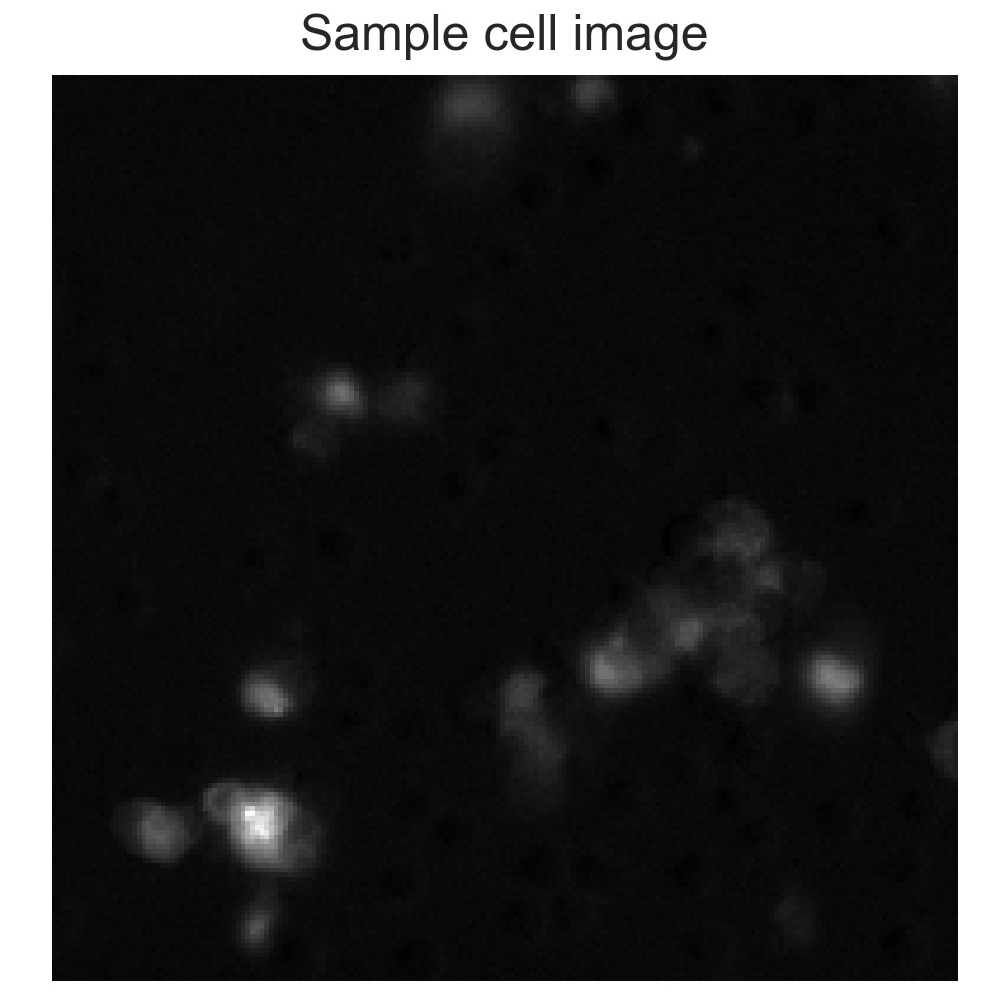
\includegraphics[width=0.6\textwidth]{dissertation/figures/sample_cell.jpg}
    \end{subfigure}
    \begin{subfigure}{0.45\textwidth}
        \centering
        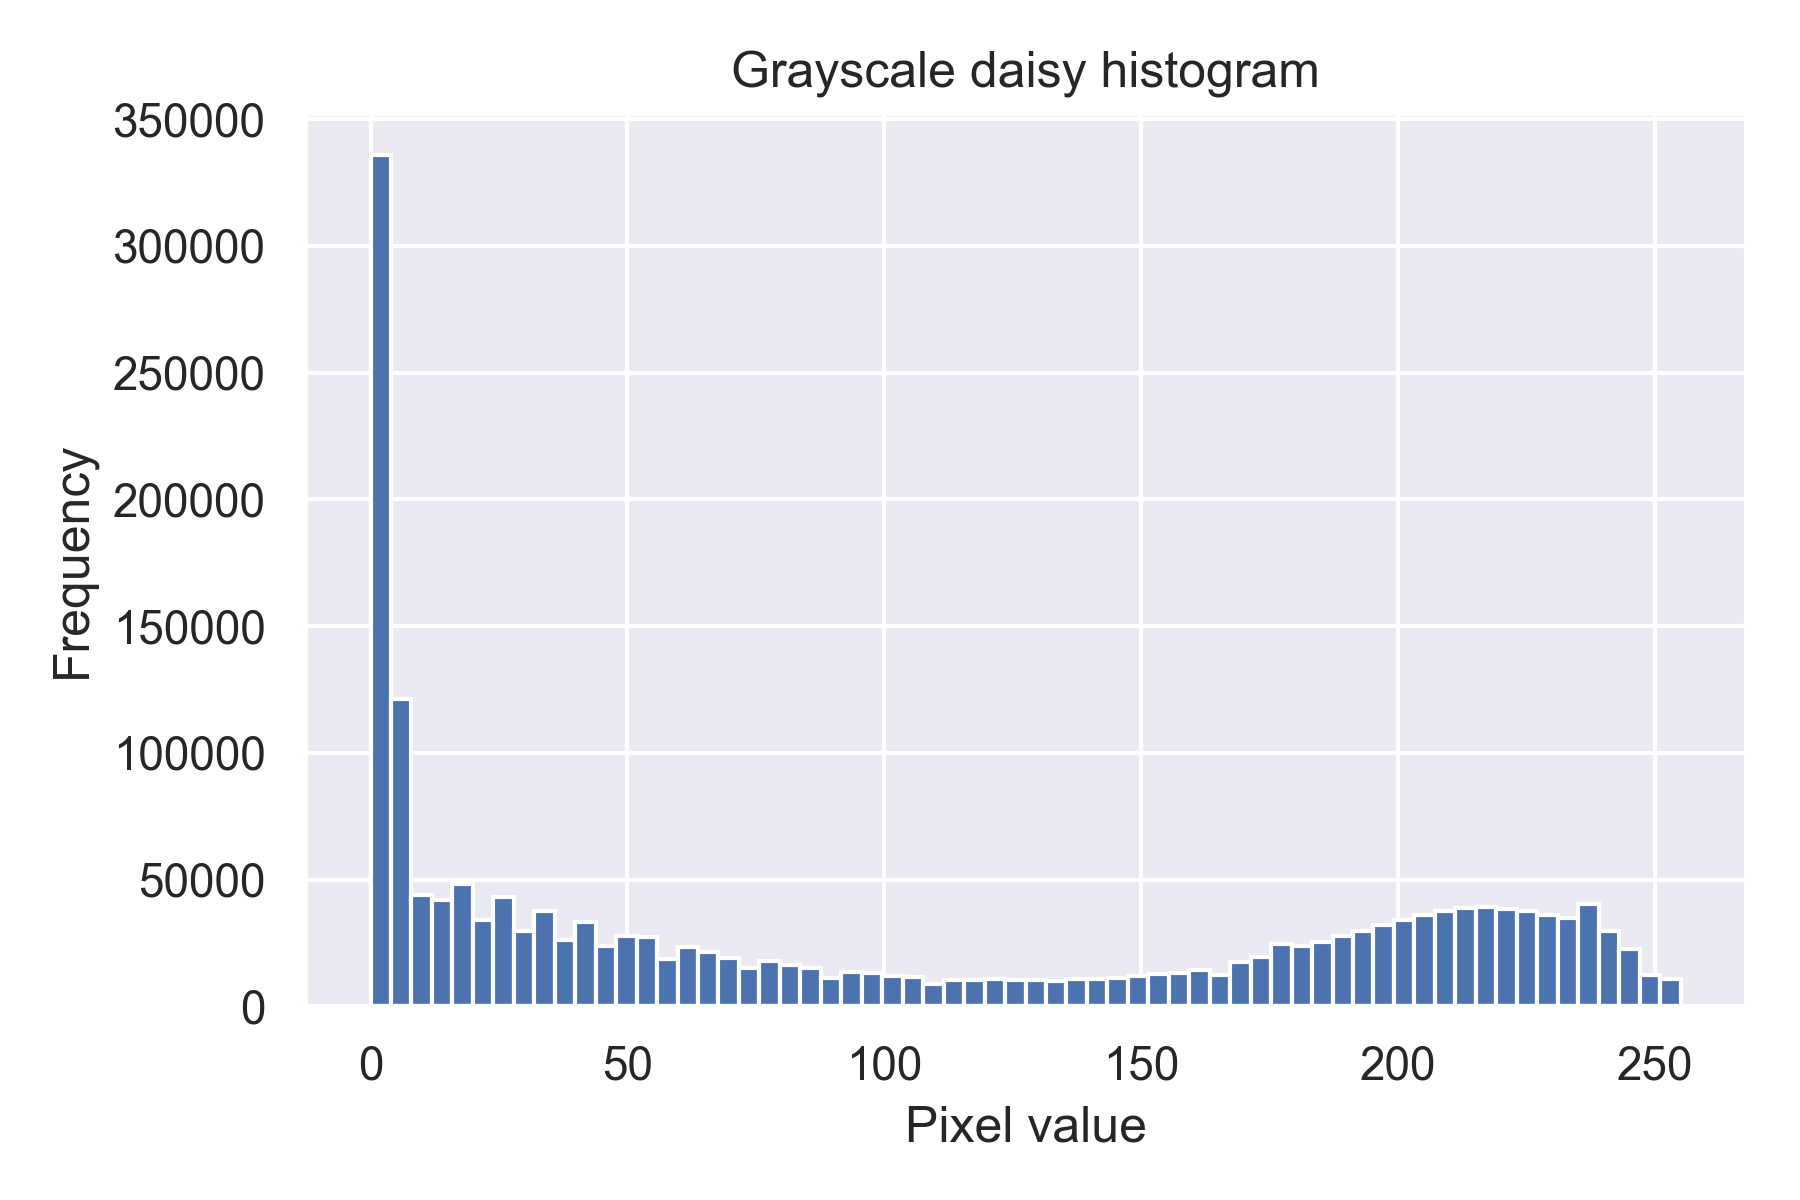
\includegraphics[width=0.8\textwidth]{dissertation/figures/grayscale_histogram.png}
    \end{subfigure}
    \begin{subfigure}{0.45\textwidth}
        \centering
        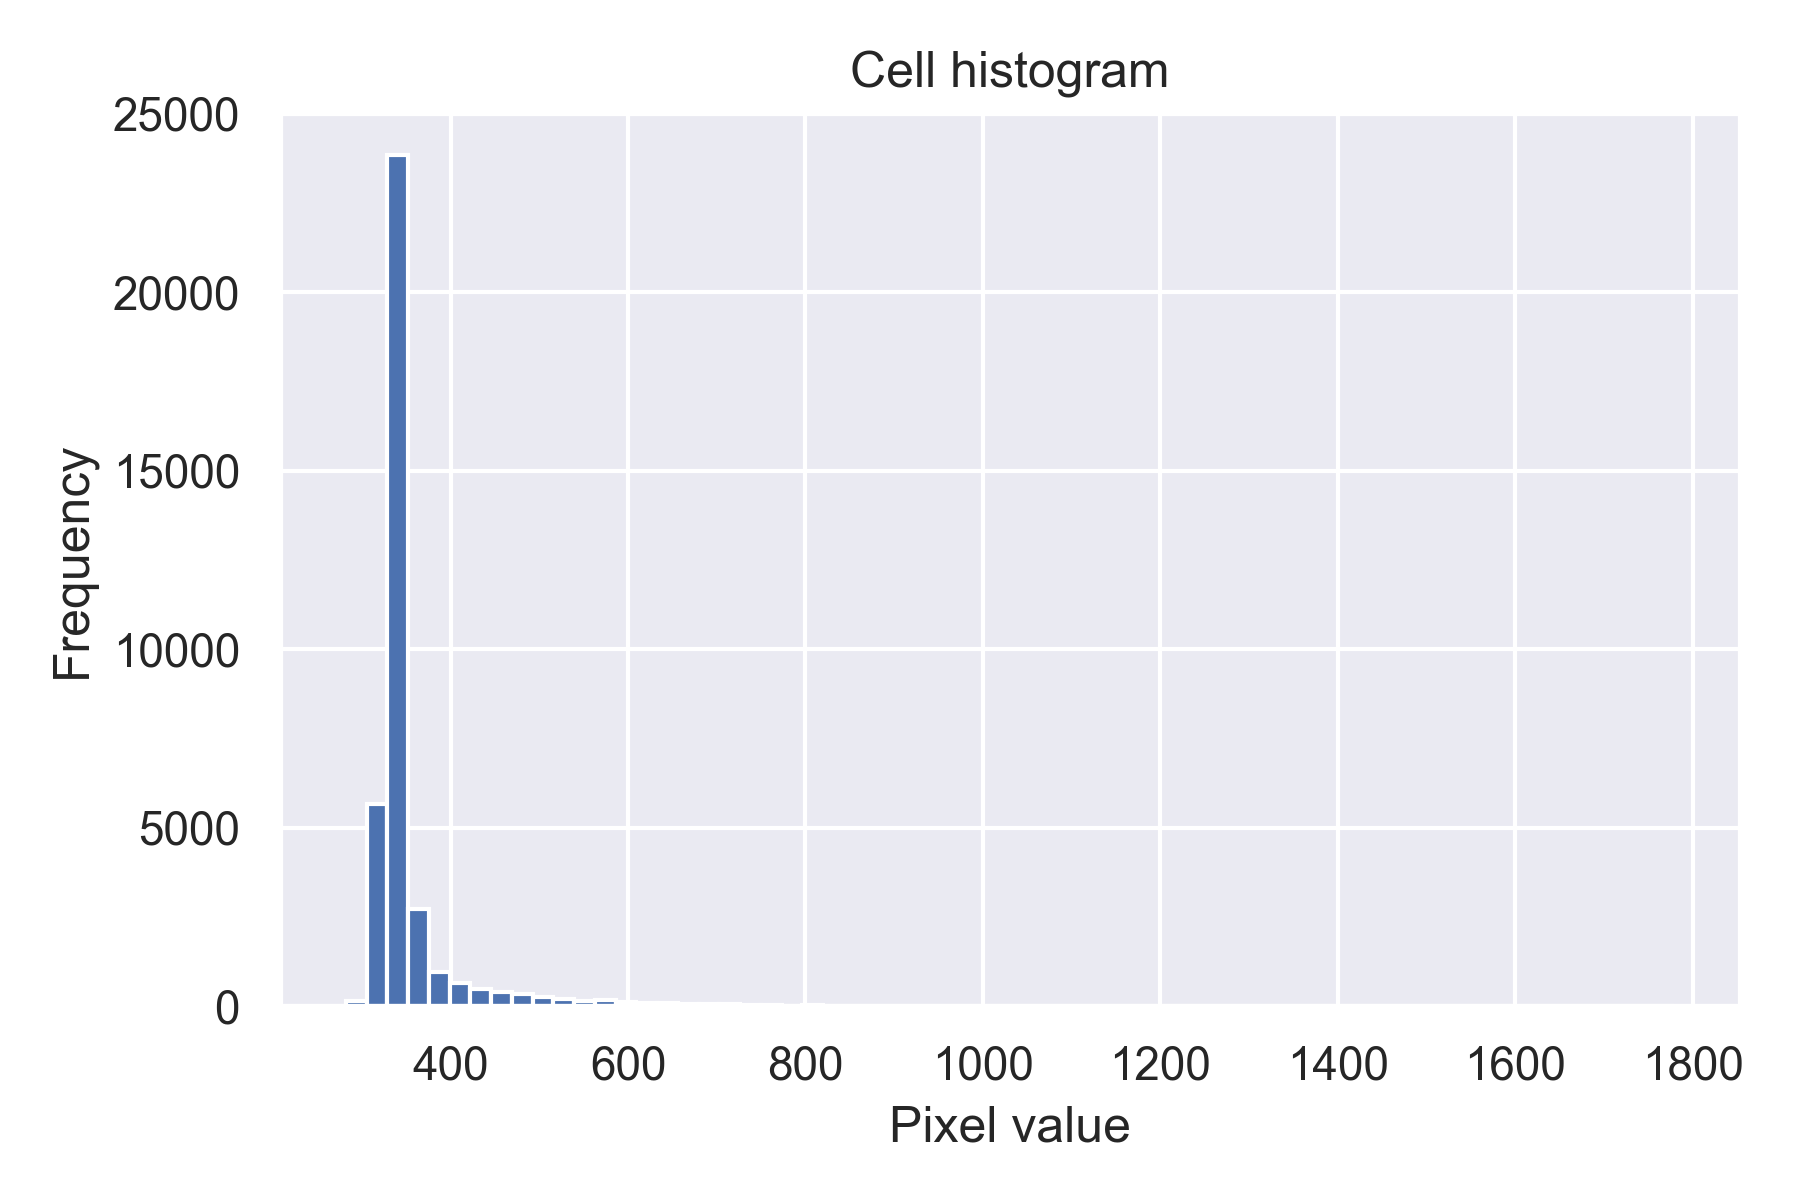
\includegraphics[width=0.8\textwidth]{dissertation/figures/cell_histogram.png}
    \end{subfigure}
    \caption{Example greyscale images and their histogram. As we can see the greyscale image of lillies has two peaks of frequency, and we can see there is a separation between the peaks at a pixel value of around 110. The greyscale image of cells has one peak, and there is a smaller frequency of pixel values past that peak, but we cannot identify a specific pixel value as a threshold from the histogram.}
    \label{fig:thresholdhist}
\end{figure}

As such, we had to find an alternative for finding a suitable threshold. First, we selected the mean pixel value as the threshold. This yielded acceptable results, however some noisy pixels still came through the mask (see Figure \ref{fig:thresholdmean}). To fix that problem, the threshold value was set as the sum of the mean pixel value and the standard deviation. This decision was based on the hypothesis that the noise level of an image with a flat structure can be estimated from its variation. Results were satisfactory, as shown in Figure \ref{fig:thresholdstd}. 

\begin{figure}[h]
    \centering
    \begin{subfigure}[h!]{0.4\textwidth}
        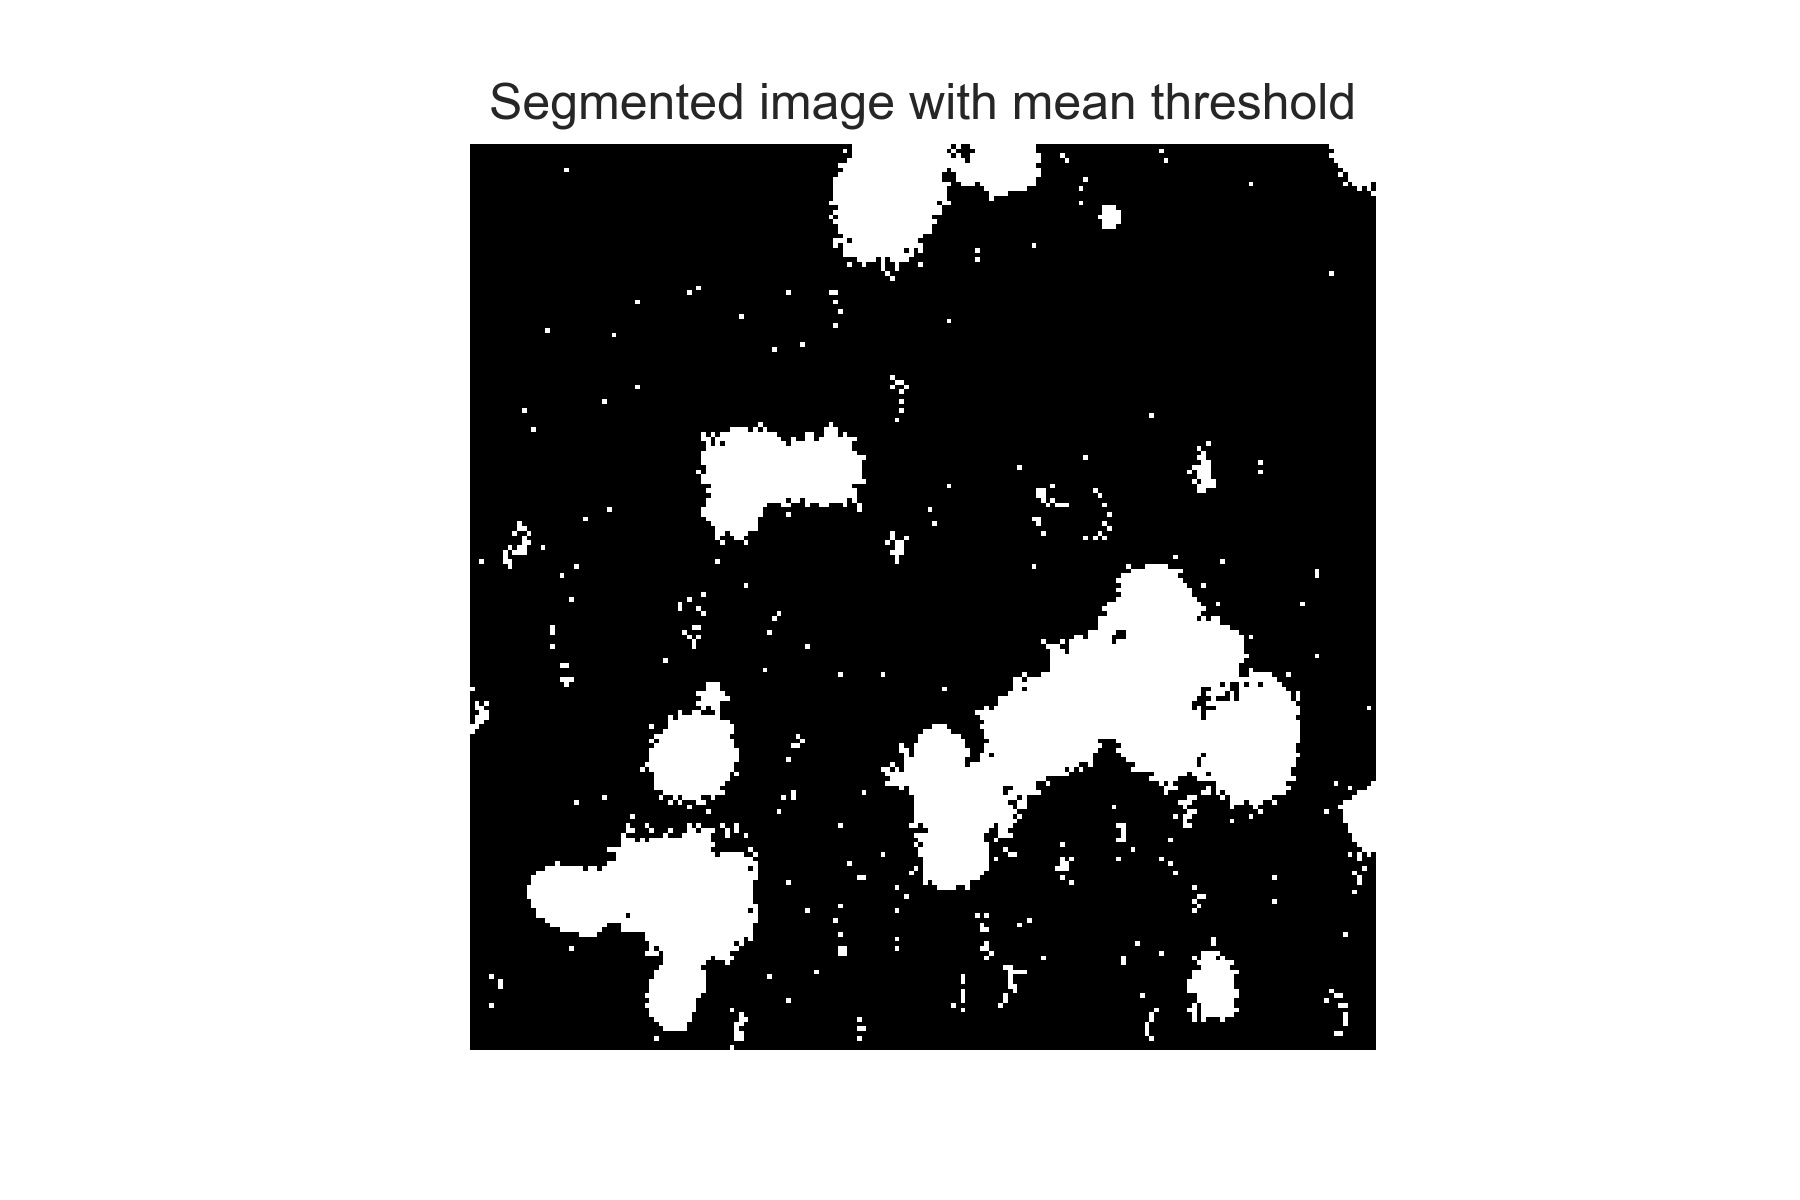
\includegraphics[width=\textwidth]{dissertation/figures/mean_threshold_cell.jpg}
        \caption{Threshold: mean pixel value}
        \label{fig:thresholdmean}
    \end{subfigure}
    \begin{subfigure}[h!]{0.4\textwidth}
        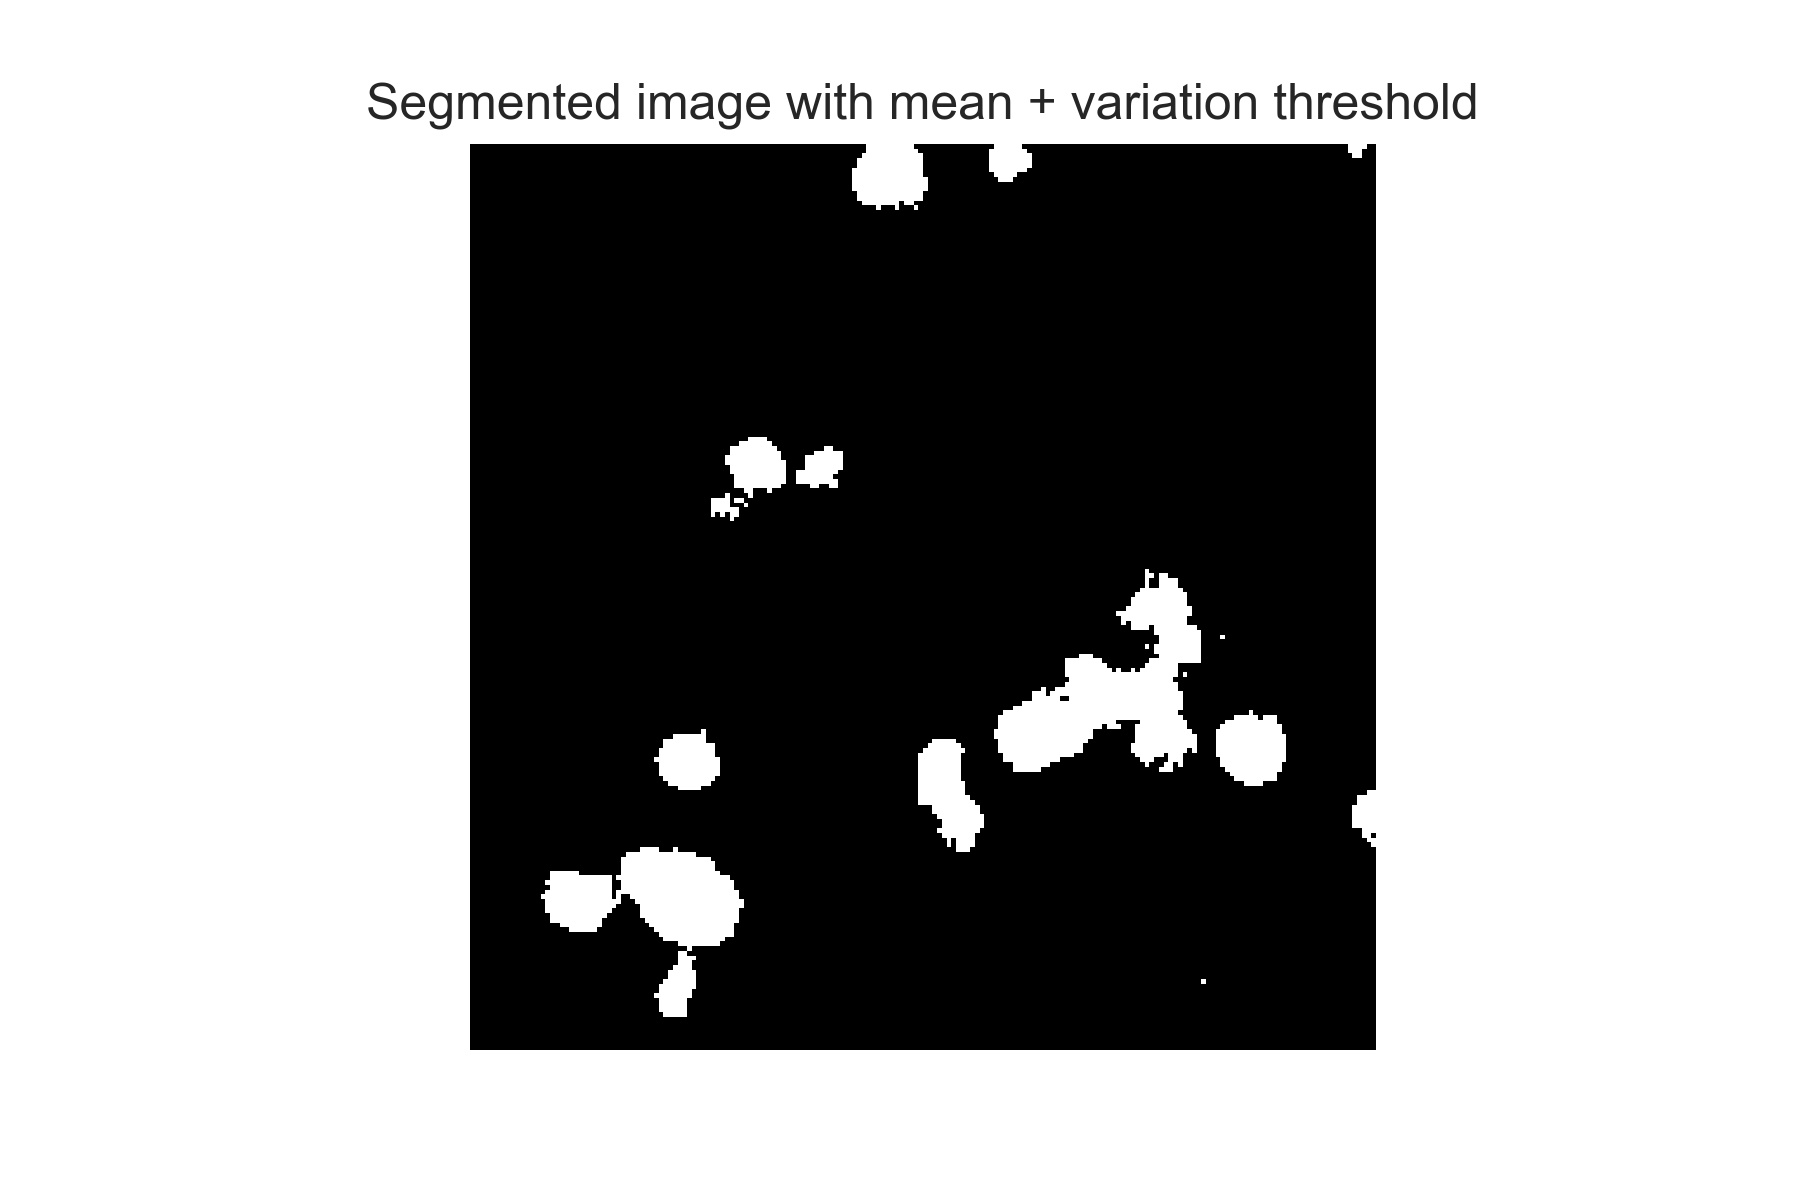
\includegraphics[width=\textwidth]{dissertation/figures/mean_std_threshold_cell.jpg}
        \caption{Threshold: mean + standard deviation}
        \label{fig:thresholdstd}
    \end{subfigure}
    \caption{Segmented images according to different threshold values. Using mean pixel value as a threshold still lets in a lot of noise in the mask, while using the standard deviation with the mean yields a much cleaner result.}
\end{figure}

Image segmentation through thresholding is also much faster than k-means, with 1,000 images being processed in 1.11 seconds with the use of NumPy arrays. That is a 26x speedup on k-means's OpenCV performance. Nonetheless, masks yielded by k-means are more granular. Figure \ref{fig:maskdiff} shows the difference between the masks obtained through different methods. 

\begin{figure}[h]
    \centering
    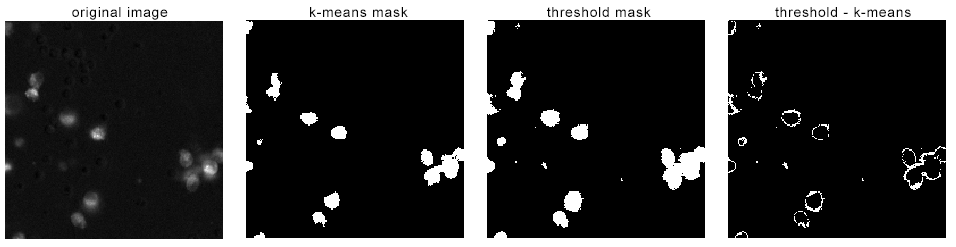
\includegraphics[width=\textwidth]{dissertation/figures/mask_difference.png}
    \caption{Different versions of the same image showing, from left to right: the original image, the k-means mask of the image, the thresholded mask of the image, and the difference between the k-means and the threshold mask.}
    \label{fig:maskdiff}
\end{figure}

\subsection{U-Net}

The U-Net model is a convolutional neural network developed for the purpose of segmenting biomedical data \citep{ronneberger_unet_2015}. It is particularly useful for labelling biomedical data when images contain multiple types of cells which have not been previously separated through the use of markers such as fluorescent dyes. Moreover, U-Net models make use of data augmentation to cope with small datasets of biomedical data. 

In our case, we do not need to segment the T cells from DCs as they have already been separated by the use of dyes. However, we wanted to compare the performance of simpler U-Net models trained to predict the mask of a greyscale image to the more traditional segmentation methods described in the sections above.

\begin{figure}[h!]
    \centering
    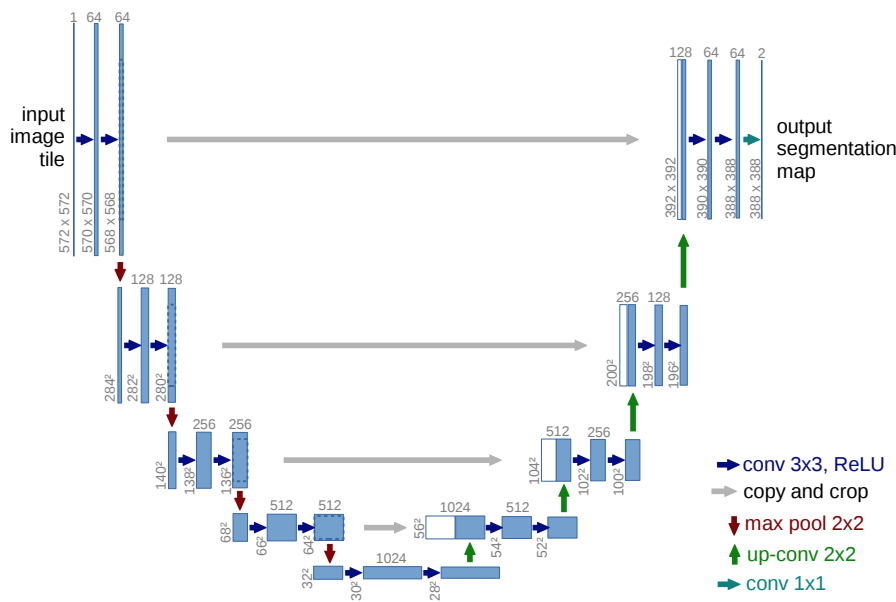
\includegraphics[width=0.6\textwidth]{dissertation/figures/unet_model.png}
    \caption{Schematic diagram of the U-Net model. The name of the model comes from its `U' structure, with an expansive path and a contracting path. Each blue rectangle represents a multi-channel feature map obtained through the network's operations. White rectangles are copied feature maps. The arrows show different operations. Source: \citet{ronneberger_unet_2015}}
    \label{fig:unet}
\end{figure}

We trained a simple U-Net model\footnote{https://www.depends-on-the-definition.com/unet-keras-segmenting-images/} on a sample of our full dataset. The input images were the \textbf{uncombined} images of T cells and DCs, and the input labels were the masks of the input images obtained with OpenCV's k-means. Training was done on 16,000 samples and validation was done on 4,000 samples of uncombined images. Training the model took 24 minutes for 20 epochs on a Google Colaboratory notebook. We then saved the model's weights and timed the generation of masks for 1,000 of the validation samples on the same machine on which we tested the k-means and thresholding methods. It took 3 minutes and 3 seconds on the machine with a CPU. With Google's GPU backend, this took 1.82 seconds. 

To conclude on all these segmentation techniques, thresholding was the fastest, with k-means coming second for CPU machines. We picked k-means with k-means++ initialisation for the granularity and satisfactory performance across all machines.

\section{Autoencoder and regression models}

\subsection{Experimental setup}

As this is a research project based on using deep learning models, a large part of the research involved an iterative process of repetitively tweaking the deep learning models, training them, and evaluating them. Immunology experiments produce a lot of imaging data, and we wanted our models to perform well on unseen data. Moreover, not all of our selected datasets contained instances of all classes. We wanted our trained model to be able to deal with such datasets too. As such, we selected the full dataset containing instances for all classes for training our model (see Table \ref{table:datasets}). Part of it was set out for validation and testing. The other two selected datasets were used purely for testing. Table \ref{table:splits} reports the number of samples in each dataset. 

\begin{table}[h]
\centering
\caption{Train-test-validation splits for selected datasets. Models are only to be trained on the full dataset. The validation set represents 15\% of the training set. The dual and DMSO-only dataset images were only used for testing.}
\rowcolor[HTML]{EFEFEF} 
\begin{tabular}{|l|r|r|r|}
\hline
\rowcolor[HTML]{EFEFEF} 
Dataset       & Train  & Validation & Test   \\ \hline
Full & 16,490 & 2,910      & 10,000 \\
Dual   &     N/A   &     N/A       & 13,900 \\
DMSO       &     N/A      &        N/A       & 8,000  \\ \hline
\end{tabular}
\label{table:splits}
\end{table}

All deep learning development was done using Keras\footnote{https://keras.io} on a Tensorflow backend. Training was carried out on Google Colaboratory notebooks\footnote{https://colab.research.google.com/} to be able to accelerate computations with Google's GPUs. 

We chose the \textit{adam} optimizer for training \citep{kingma2014method}. While training, we used Keras's callbacks feature to monitor the model's validation loss and change training parameters accordingly. The model would reduce its learning rate by a factor of 0.2 if no improvements in the validation loss were seen over 3 epochs (i.e. the model entered a plateau), and we used early stopping to stop training if no improvements were witnessed in validation loss over 5 epochs. Training was usually ran with a batch size of 64 over 40 epochs. 

\subsection{Convolutional autoencoder}

The main model to be developed was a convolutional autoencoder. The autoencoder was built for two purposes: obtaining a smaller representation of each of the images to be fed into high-dimensional visualisation algorithms, and to be the building block for a deep regression model.

An autoencoder follows a symmetrical structure of reduction and expansion operations. The reduction operations represent the encoding part of our model, and the expansion operations represent the decoding part of our model. In order for the autoencoder input to be reduced and then reconstructed to the same number of input dimensions, we need the two sets of operations to follow the same pattern and use the same number of parameters. Figure \ref{fig:symmstruc} illustrates the symmetrical structure of an autoencoder, and shows the core layers of a convolutional autoencoder: convolution layers combined with activation functions, and pooling/upsampling layers.

\begin{figure}[h!]
    \centering
    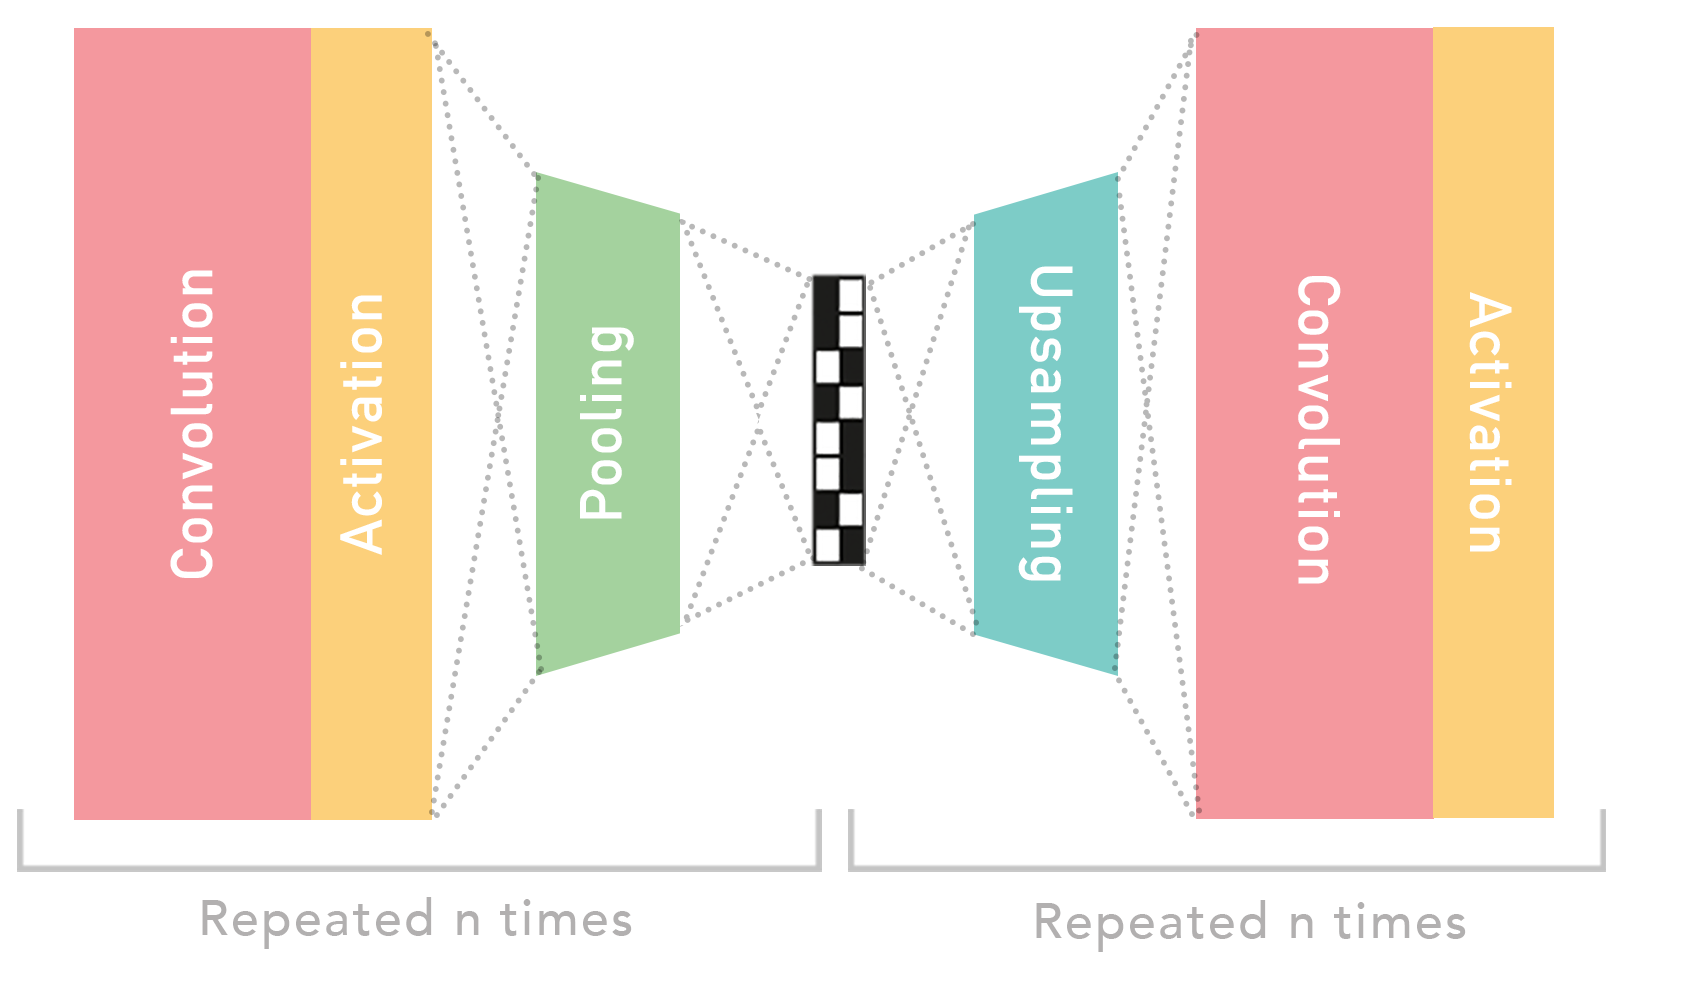
\includegraphics[width=0.6\textwidth]{dissertation/figures/autoencoder_repeat_structure.png}
    \caption{Diagram for a typical autoencoder structure. Operations are repeated the same amount of times in the reductive path and the expansive path for the input to be reconstructed with the same dimensions at the output. Convolution layers are used with an activation function, and followed by a pooling operation in the reductive path, and preceded by an upsampling operation in the expansive path. The bottleneck layer holds a smaller representation of an image.}
    \label{fig:symmstruc}
\end{figure}

\textit{Convolution} refers to the process of taking the weighted sums of neighbouring values. Convolutional layers can be thought as a window sliding over an image and summing everything within that window. The specific behaviour of a convolution operation is determined by the filter it uses. Each element in the window will be multiplied by the corresponding element of the filter. We can specify both how big the filter should be, as well as how many different filters should be used. If we use 64 filters, we will learn 64 features about the image, but it will also multiply our dimensions by 64. Figure \ref{fig:convolution} illustrates the convolution process. The values of the filters are parameters to be learned by the model. 

\begin{figure}[h]
    \centering
    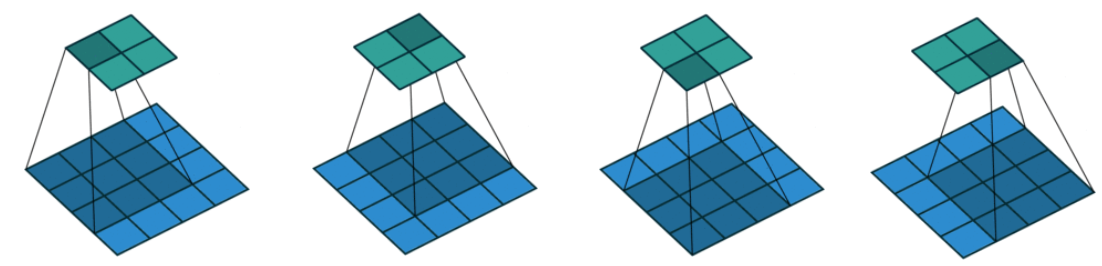
\includegraphics[width=0.6\textwidth]{dissertation/figures/convolution_operation.png}
    \caption{Step-by-step illustration of a simple $3\times3$ convolution operation on a $4\times4$ image, resulting in 4 convolution features. Source: \citet{dumoulin2016guide}}
    \label{fig:convolution}
\end{figure}

\textit{Activation functions} define whether or not each element in the output of the convolutional layer (in this case) should be set to `on' or `off'. The purpose of an activation function is to only `activate' elements of the hidden layers' outputs if it seems to be contributing to the learning of the model. Activation functions transform an input to an output according to their definition so they have to be chosen accordingly.

\textit{Pooling layers} will downsample an image by passing a window over an image and selecting a set value from that window as the one to keep. There are two main types of pooling operations commonly used: average pooling and maximum pooling. In average pooling, the mean value of a window will be chosen as output. In maximum pooling, the maximum value of a window will be chosen. Their counterpart are \textit{upsampling layers} which will resize an image to the right dimensions for a convolutional operation to be applied to it. An illustration of the how these layers function is provided in Figure \ref{fig:sampling}. Using a combination of upsampling and convolutional layers is an alternative to using deconvolution layers which have the drawback of creating checkerboard artifacts \citep{odena2016deconvolution}.

\begin{figure}[h!]
    \centering
    \begin{subfigure}{0.45\textwidth}
        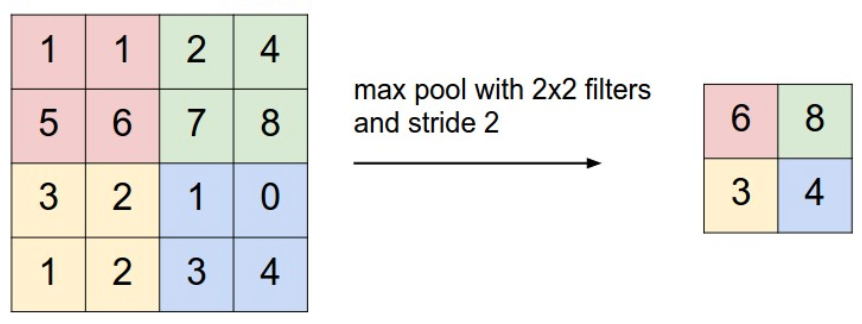
\includegraphics[width=\textwidth]{dissertation/figures/pooling_operation.png}
        \caption{Pooling}
    \end{subfigure}
    \begin{subfigure}{0.45\textwidth}
        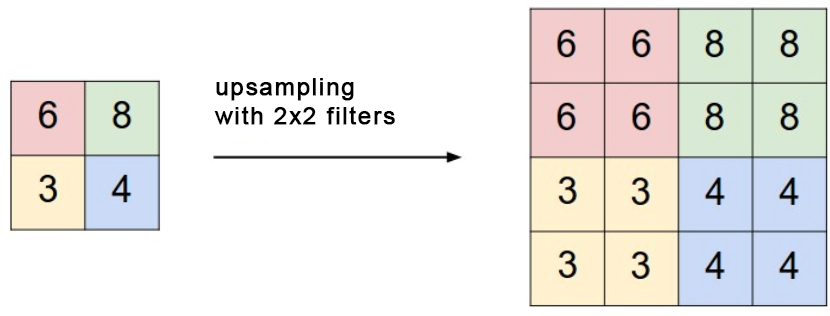
\includegraphics[width=\textwidth]{dissertation/figures/upsampling_operation.png}
        \caption{Upsampling}
    \end{subfigure}
    \caption{Left: maximum pooling of $2\times2$ with stride of 2 applied to a $4\times4$ image. The image is reduced by a factor of 2. Right: upsampling of $2\times2$ with stride of 2 applied to a $2\times2$ image. The image is augmented by a factor of 2. Adapted from \citet{karpath_cs231n}.}
    \label{fig:sampling}
\end{figure}

Throughout the development of the autoencoder, the aim was to maximise the reduction of dimensionality while maintaining a satisfactory reconstructed image. A trade-off had to be done as quality decreases with the decrease of dimensionality. Size of the coded representation was mainly impacted by the number of hidden layers and size of the convolution and pooling filters. Quality of the reconstructed image could be improved with larger features being used in the convolutional layers and smaller filters. 

\bigskip
\subsubsection{Implementation choices}
\hfill 
\hfill 

Knowing this, the structure of the autoencoder was tuned by trial and error and literature review of existing neural networks for similar applications.

In order to avoid losing too much detail in the reconstructed image, we only used $3\times3$ filters in convolution layers and pooling was done by a factor of 2. Moreover, we kept the number of features retrieved by convolution layers relatively high (64 -> 32) so as not to lose too much detail in the images. Our structure also used decreasing filter size instead of increasing filter size. Even though increasing filter size showed slight improvements in reconstruction, they were minimal, and having bigger filters towards the bottleneck layer generated bigger coded dimensions.

We also decided to replace the pooling operation in the last layer before the bottleneck by a strided convolution layer. \citet{springenberg_striving_2014} show that adding striding to convolution layers instead of using pooling operations can achieve the same levels of accuracy. Furthermore, by adding the downsampling operation to the convolution layer, the network will learn how to best perform this operation as convolutions are weighted layers. We did not add strides to all our convolution layers in place of pooling layers as strides do come at the performance cost of having more trainable parameters. Our experiments showed that the colours in the reconstructed image seemed slightly more detailed when using striding over pooling, but this was very minimal and the choice came down to wanting to experiment.

In the hidden layers, the choice of activation function was a variant of the Rectified Linear Unit (ReLU), the Parametric Rectified Linear Unit (PReLU). ReLU simply returns 0 if the weight unit in the output of a layer is less than 0, or the actual weight if it is bigger than 0. It has become popular because it has been shown to outperform the conventional sigmoid function in hidden layers \citep{hinton_relu, glorot2011}, as well as helping with faster training convergence \citep{krizhevsky_imagenet_2012}. PReLU differs from ReLU by having a small slope for negative values which means it does not map all negative values to 0. This slope is made a training parameter and is determined by the neural network during training. Figure \ref{fig:relu_prelu} illustrates the difference between the two. \citet{he_2015} showed that PReLU can improve model fitting for image classification applications. Reconstruction difference using PReLU over ReLU in our model is shown in Figure \ref{fig:relu_prelu_reconstruction}. Our PReLU model also had a slightly lower validation loss of 0.0871 compared to ReLU's 0.0875. 

\begin{figure}
    \centering
    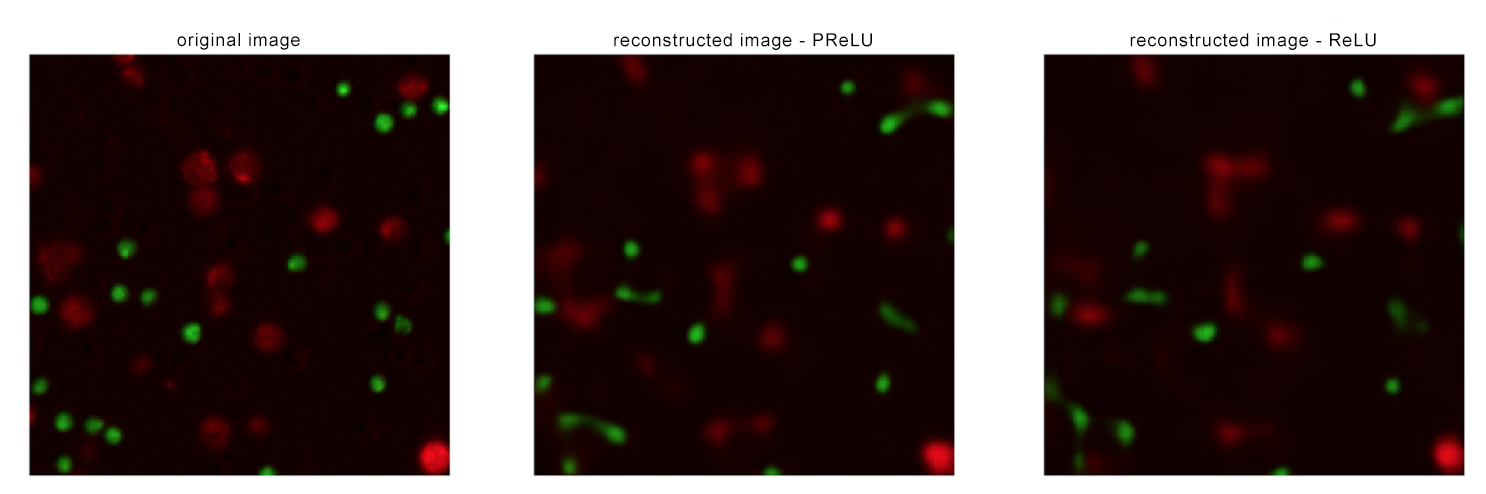
\includegraphics[width=.9\textwidth]{dissertation/figures/relu_prelu_reconstruction.png}
    \caption{Autoencoder reconstruction of validation images under different activation functions. The original image is on the left, and we can observe the difference between reconstruction with PReLU (middle) and ReLU (right).}
    \label{fig:relu_prelu_reconstruction}
\end{figure}

\begin{figure}[h!]
    \centering
    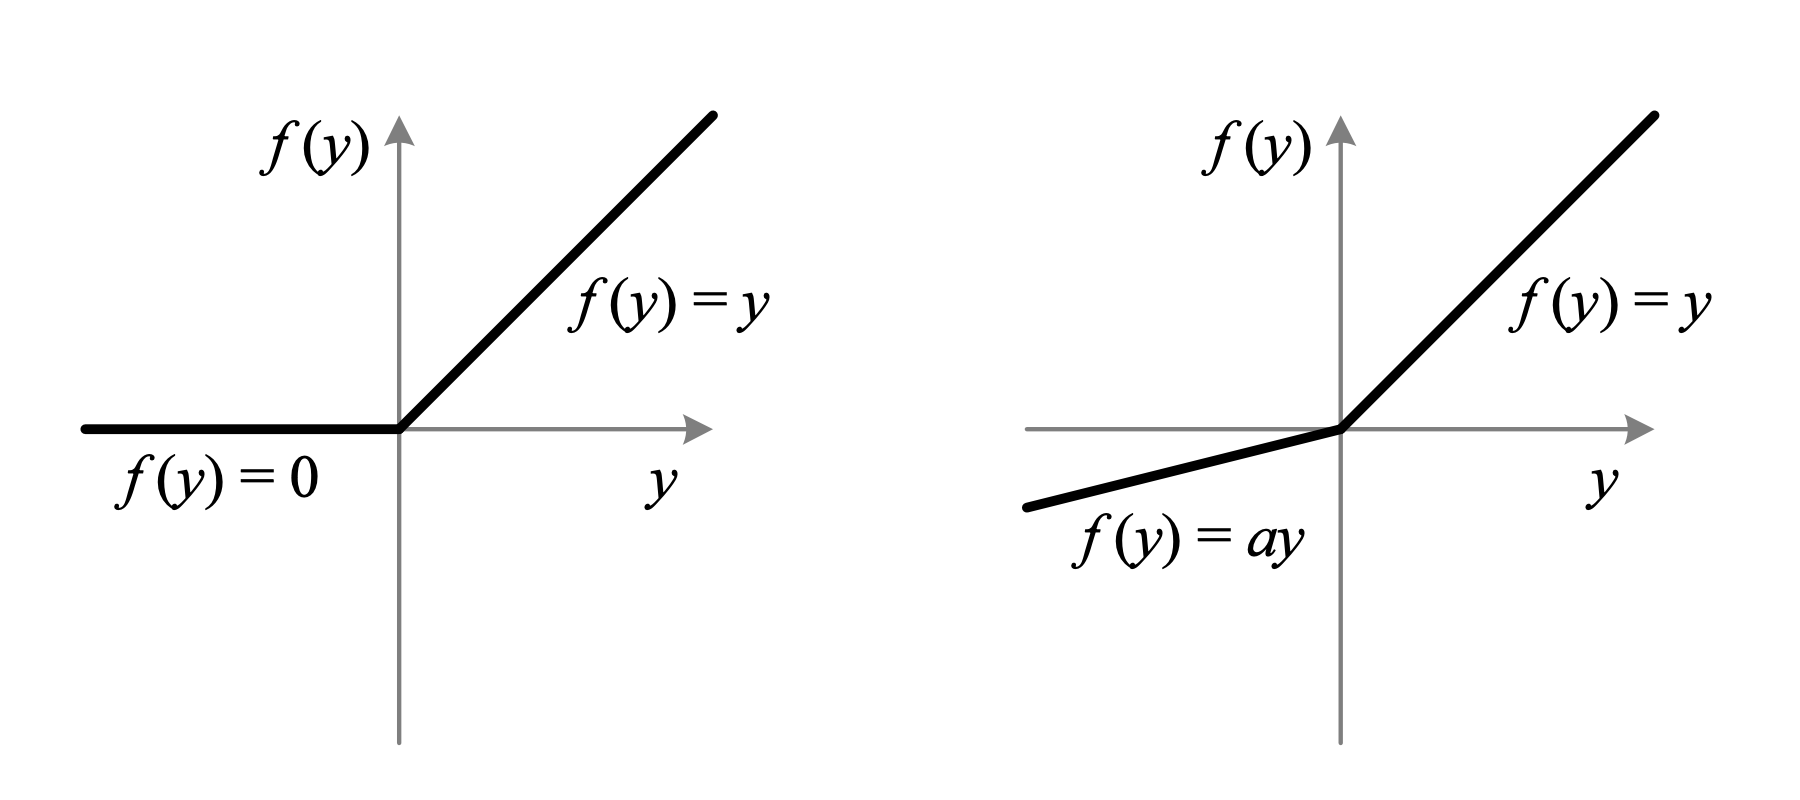
\includegraphics[width=.55\textwidth]{dissertation/figures/relu_prelu.png}
    \caption{ReLU (left) vs. PReLU (right). The negative part of the PReLU function is variable and a parameter to be learned. Source: \citet{he_2015}}
    \label{fig:relu_prelu}
\end{figure}

\begin{figure}[h!]
    \centering
    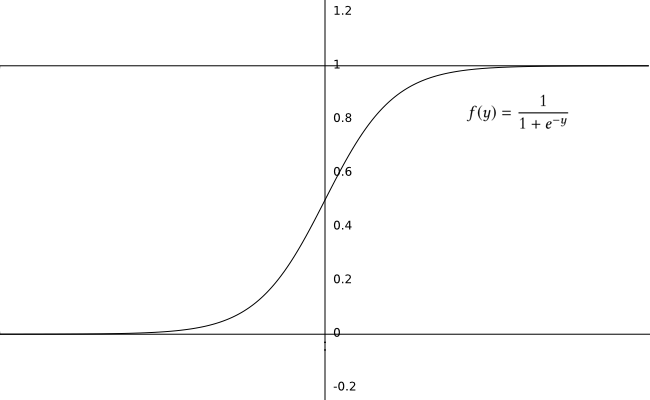
\includegraphics[width=.45\textwidth]{dissertation/figures/sigmoid.png}
    \caption{Function graph of the logistic sigmoid function. The logistic sigmoid function is characterised by its `S' shape. Any input will be bounded in [0, 1] at output.}
    \label{fig:sigmoid}
\end{figure}

The activation function at the output of the network was the logistic sigmoid activation function, as we needed to restrict output to the [0, 1] range of our image pixels. Figure \ref{fig:sigmoid} illustrates this activation function. 

Our final autoencoder structure reduced dimensions by a factor of 2 a total of 5 times, resulting in a tenfold reduction of dimensions on the original 110,592 pixels. The final coded dimensions were of 1,152. Figure \ref{fig:diff_reconstructions} illustrates how the autoencoder reconstructed an input image depending on number of pooling operations. We traded off some reconstruction quality in order to obtain a smaller coded dimension in the hope that it would help high-dimensional visualisation algorithms perform better, as well as be a better starting block for a regression model. 

\begin{figure}[h]
    \centering
    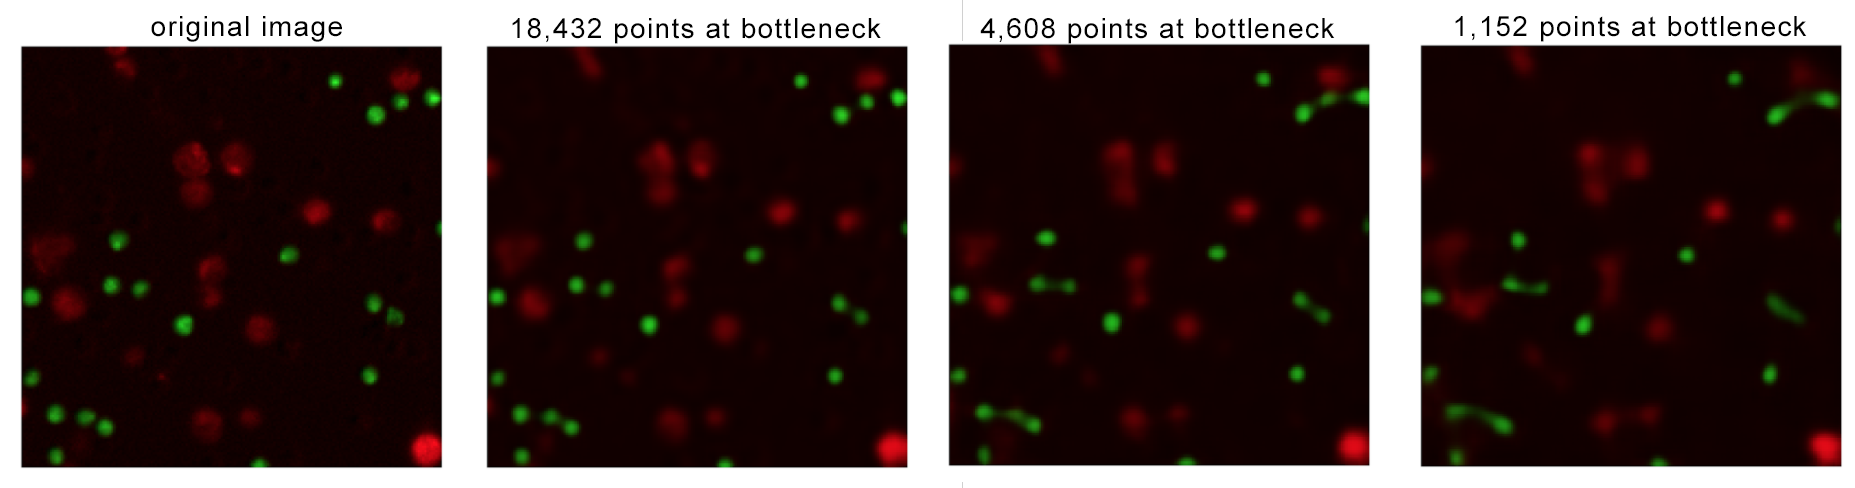
\includegraphics[width=.95\textwidth]{dissertation/figures/reduction_trade_off.png}
    \caption{Images reconstructed by the autoencoder according to the size of the coded layer. From left to right: the original image to reconstruct, the image reconstructed from 3 convolution-pooling operations, the image reconstructed from 4 convolution-pooling operations, the image reconstructed from 5 convolution-pooling operations. Quality decreases with the number of pooling operations.}
    \label{fig:diff_reconstructions}
\end{figure}

The autoencoder was trained with binary cross-entropy as a loss function, as we were aiming to minimise the difference between two distributions: the input, and the reconstructed output. The final structure of the autoencoder is shown below in Figure \ref{fig:autoencoder_details}. Keras code for building the model is available in Listing \ref{lst:autoencoder}. 

\begin{figure}[h]
    \centering
    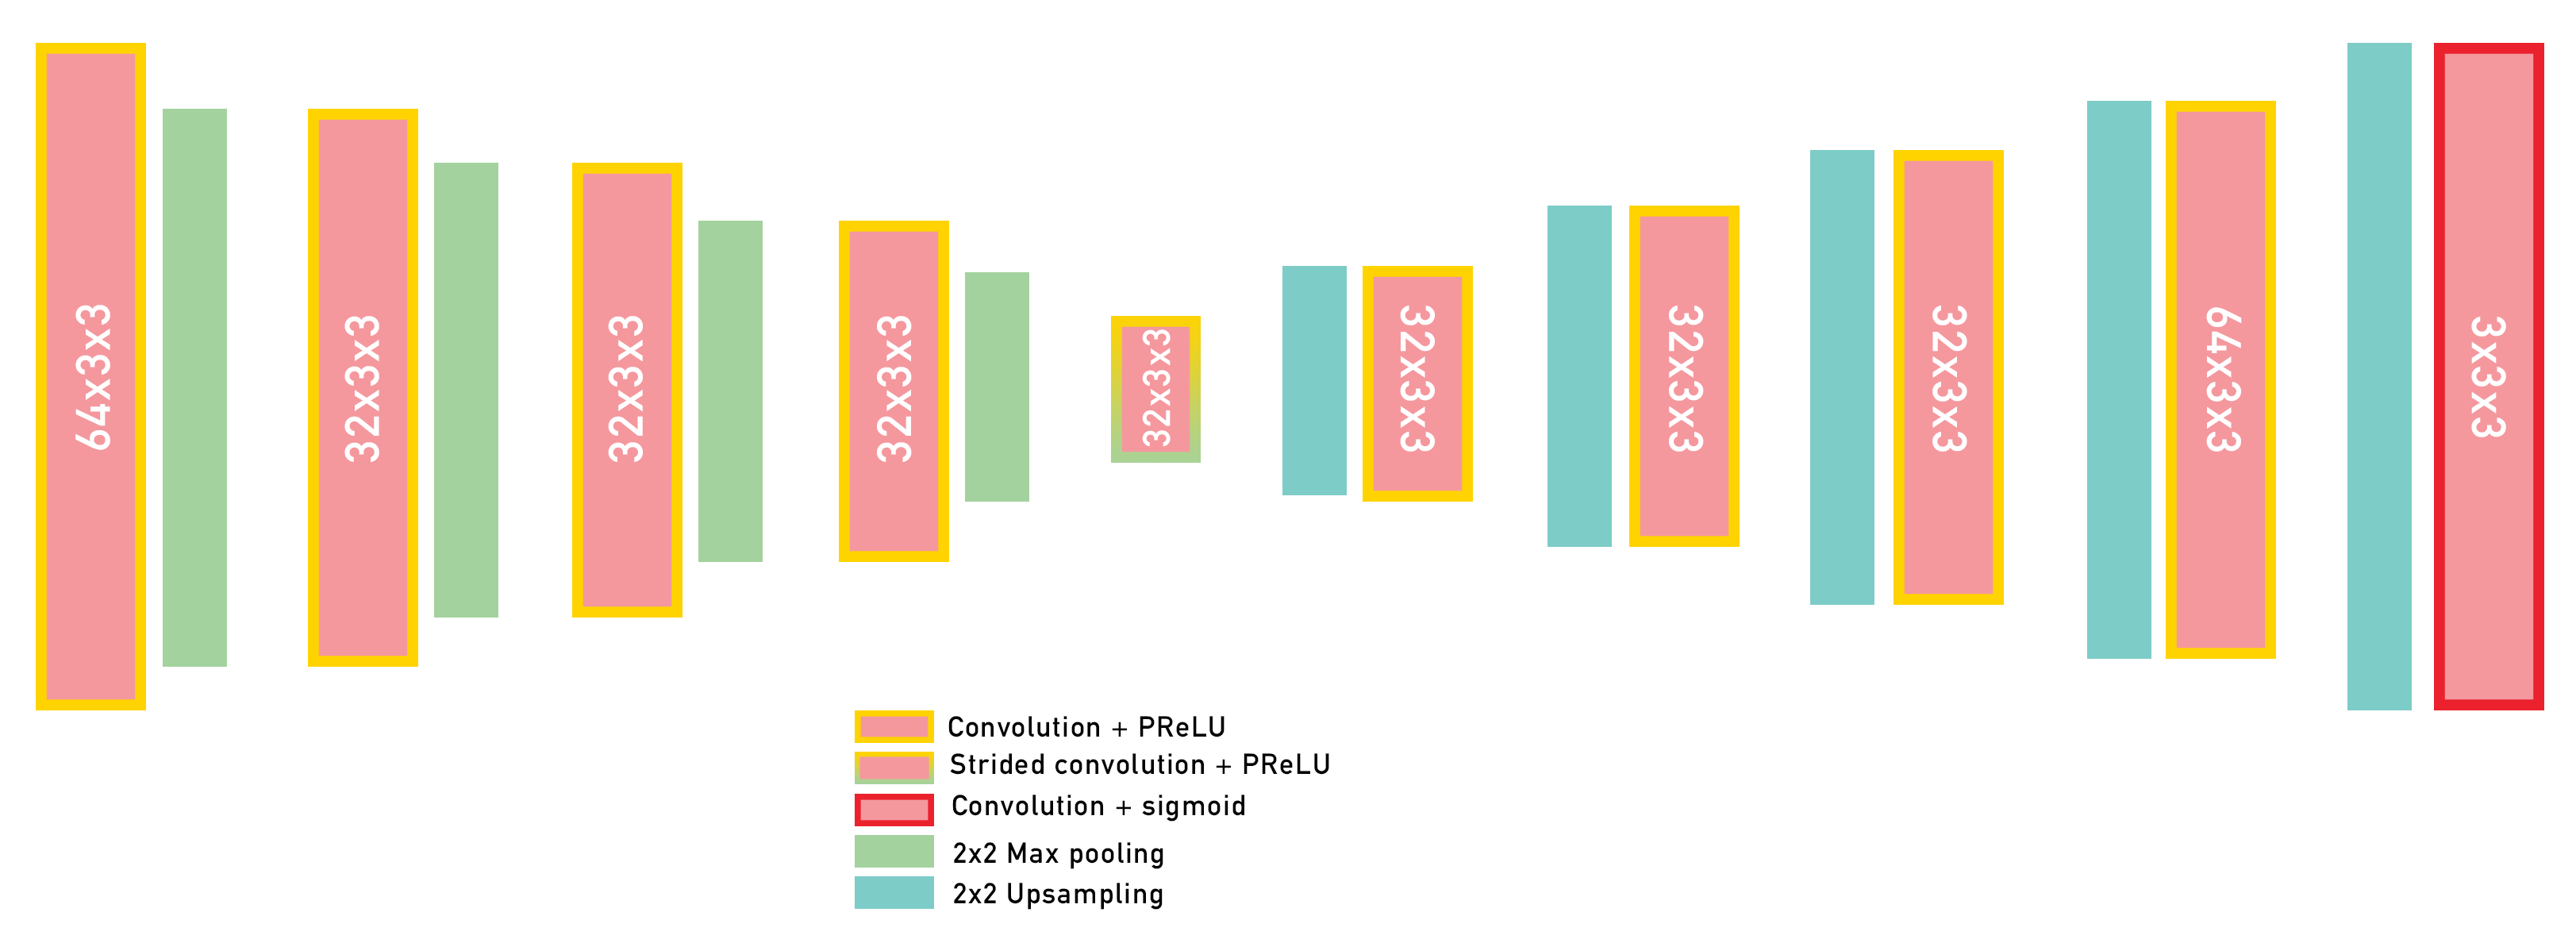
\includegraphics[width=.9\textwidth]{dissertation/figures/autoencoder_final_structure.png}
    \caption{Diagram of the final implemented autoencoder structure. Convolution blocks are represented in pink, attached to activation functions in yellow or red. Downsampling operations are in green and upsampling operations are in blue. The special strided convolution layer uses a green to yellow gradient to represent the downsampling of the striding and the activation function set in the layer.}
    \label{fig:autoencoder_details}
\end{figure}

\subsection{Deep regression}

The regression model was built on the encoder part of the autoencoder. We wanted to use the dimensionality reduction capacities of the encoder layers to evaluate whether interaction could be quantified from an image's features. 

The structure of the regression model was kept simple. Research reviewing existing general-purpose neural networks such as VGG-16 showed that adequate tuning of these models resulted in a performance close to ``state-of-the-art'' without having to develop more complicated structures \citep{Lathu2018}. We did not reuse such a general purpose model but the convolutional part of the VGG-16 network is similar to the encoder part of our autoencoder, using 5 combinations of convolutions and pooling operations. These operations are followed by a small number of fully-connected layers \citep{Simonyan15}. Hence, we decided to follow this template and not make our regression structure overly complex.

The encoder model was extracted from the autoencoder with the bottleneck layer flattened. This encoder model was then extended with two fully connected layers separated by a dropout layer. The fully connected layers were activated by ReLU. Dropout layers are used to randomly turn some units of the output of hidden layers to 0. Dropout was shown to make models more robust and prevent overfitting \citep{hinton_improving_2012}. The final regression predictions were outputted with a fully connected layer of size 1, activated by a linear function. 

The choice of the linear function was justified by the following. The input to the regression model was $192\times192\times3$ images accompanied with labels in the range [0, 100] representing a percentage of overlap between two groups of cells. As such, we want the output activation function to be limited to [0, 100]. Both softplus and linear activations were candidates. The linear activation had to be used with a non-negative kernel constraint, as overlap percentage cannot be negative but the linear function normally allows for negative values. The softplus activation function outputs values in the range [0, $+\infty$]. Performance in terms of training loss was similar, however the linear function performed overall better. Furthermore, softplus does not always map an input to itself around 0 (shown in Figure \ref{fig:linear_softplus}) and is harder to differentiate compared to the linear function, which would make training slower.  

\begin{figure}[h]
    \centering
    \begin{subfigure}{0.4\textwidth}
        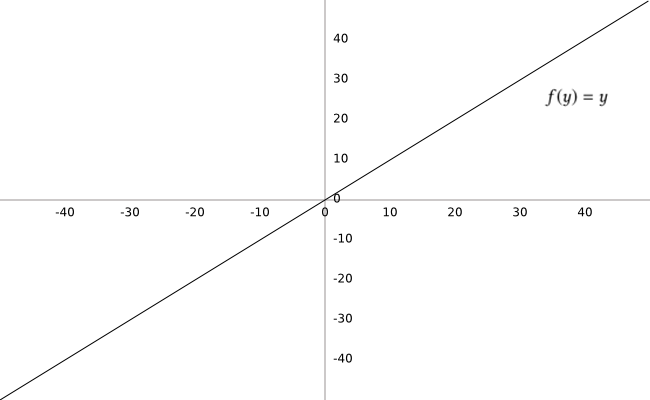
\includegraphics[width=\textwidth]{dissertation/figures/linear_function.png}
        \caption{Linear}
    \end{subfigure}
    \begin{subfigure}{0.4\textwidth}
        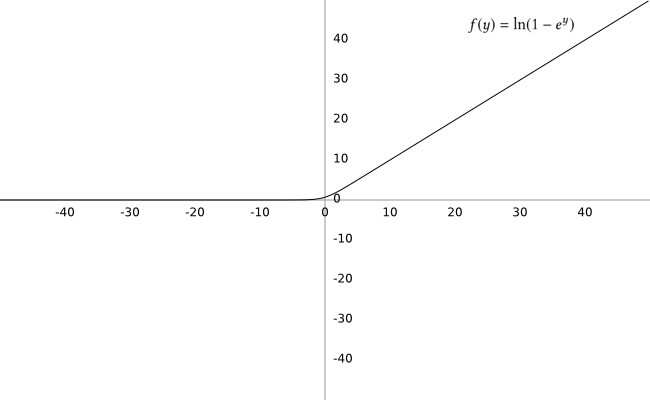
\includegraphics[width=\textwidth]{dissertation/figures/softplus_function.png}
        \caption{softplus}
    \end{subfigure}
    \caption{Function graphs of the linear function (left) and the softplus function (right).}
    \label{fig:linear_softplus}
\end{figure}

The regression model was trained with mean-squared-error loss, which calculates the difference between the predictions of the model and the truth values of the labels. The final structure of the deep regression model is shown in Figure \ref{fig:regression_details}. Keras code for building the model is available in Listing \ref{lst:regression}. 

\begin{figure}[!ht]
    \centering
    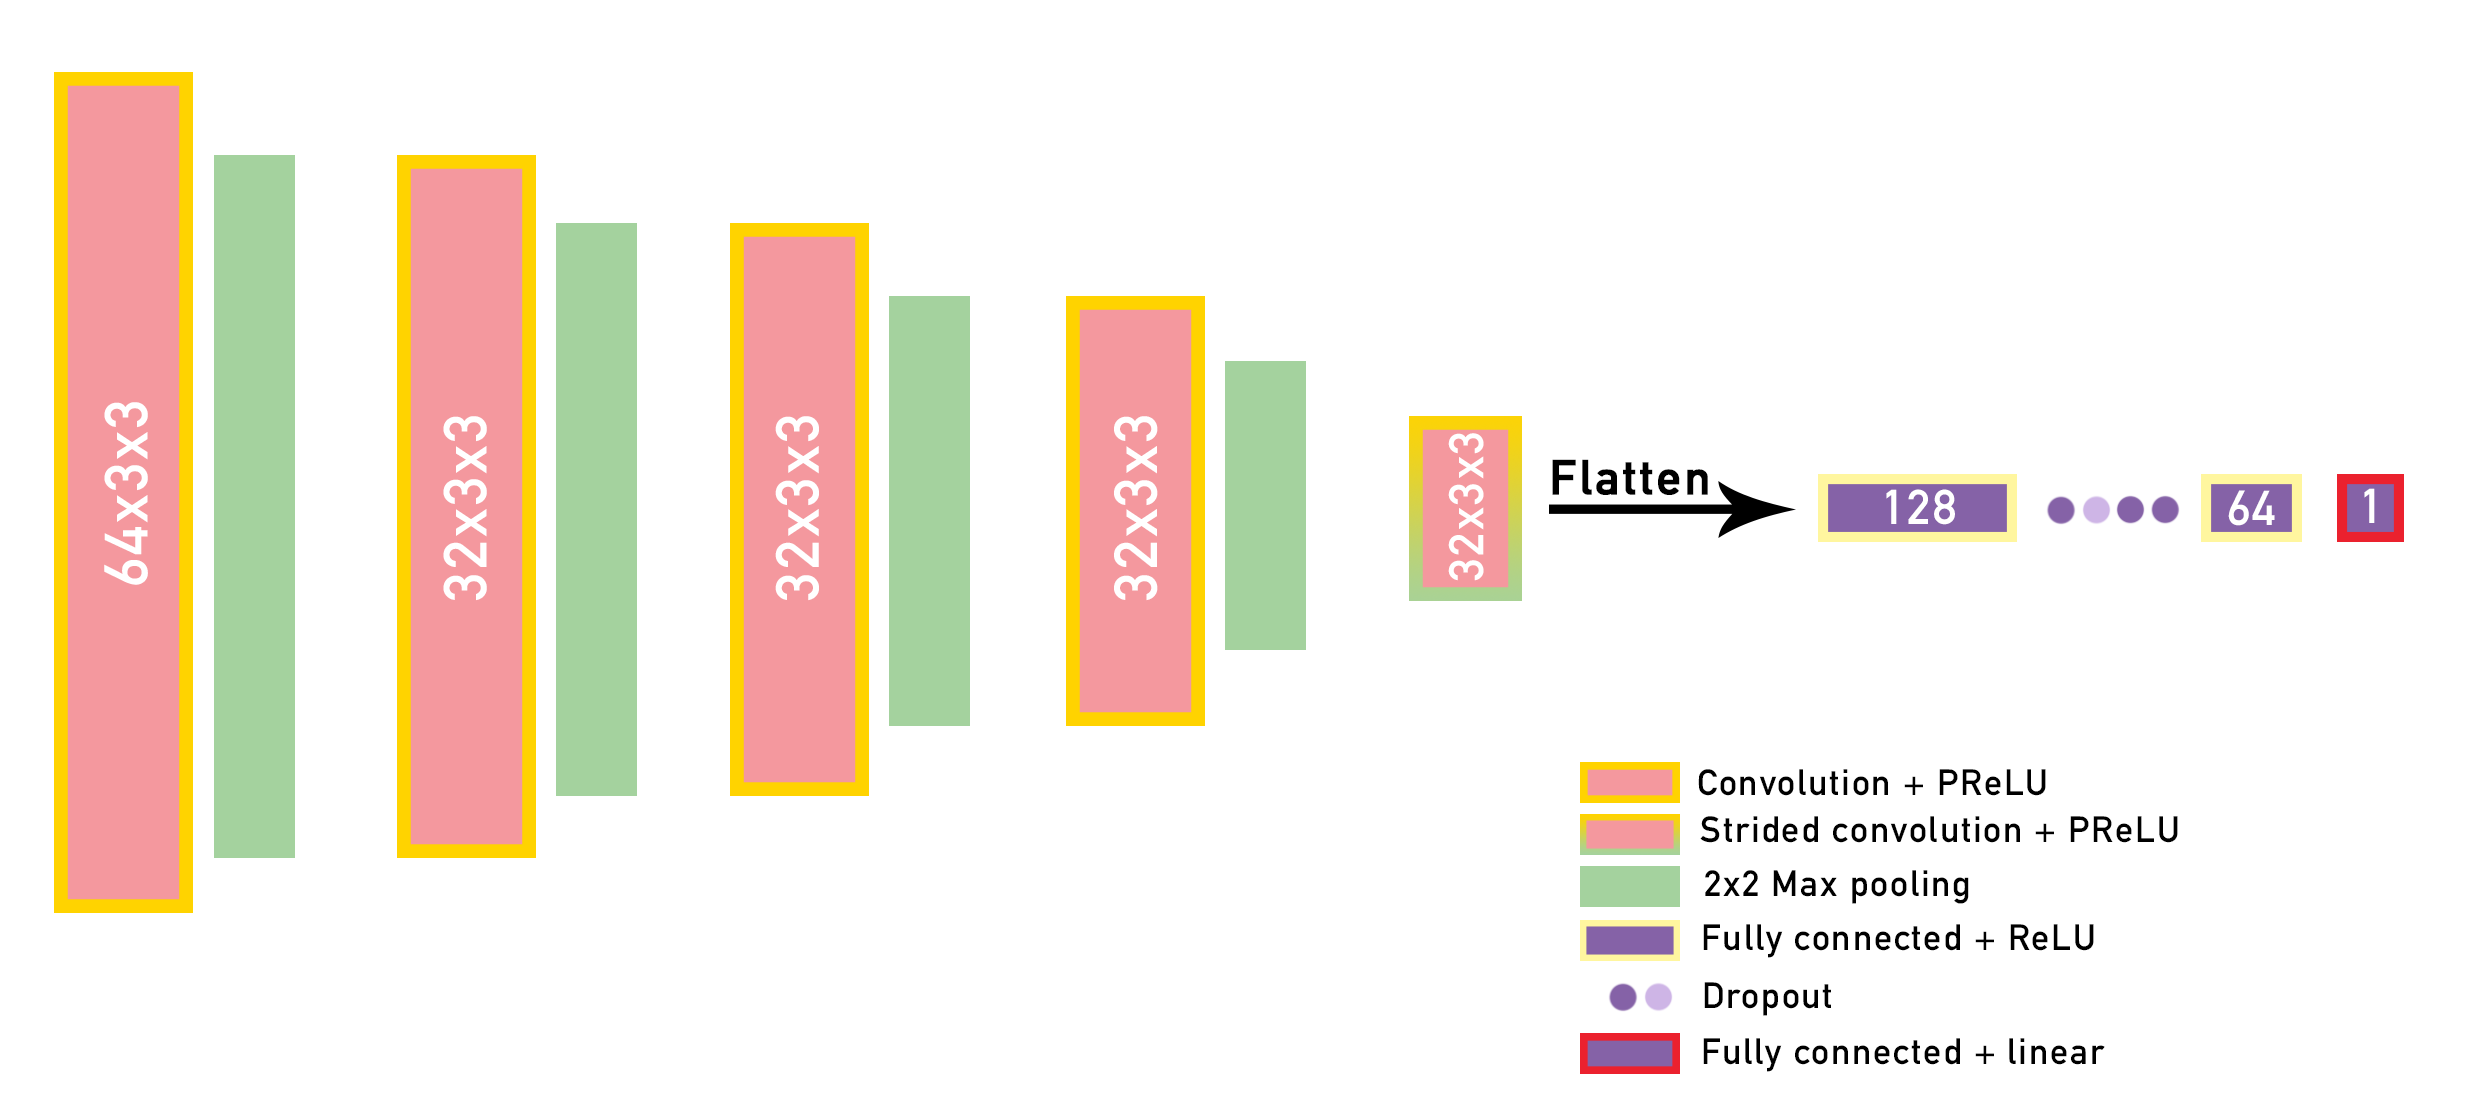
\includegraphics[width=.85\textwidth]{dissertation/figures/regression_final_structure.png}
    \caption{Diagram of the implemented regression structure. Note that the first part of the diagram is the exact same as the contracting path of the autoencoder shown in \ref{fig:autoencoder_details}, but the output of the strided convolutional layer is flattened and passed onto fully connected layers. Fully connected layers are purple rectangles, and the Dropout layer is shown by purple dots. Activation functions are represented in yellow or red.}
    \label{fig:regression_details}
\end{figure}